\section{Incentivization Mechanism}
\label{sec:incentiviationmechanism}

The HOPR protocol provides incentives to nodes in the network to achieve correct transformation and delivery of mixnet packets. This is accomplished through a combination of \lcnameref{sec:proofofrelay}, a novel mechanism which is cost effective and privacy preserving, and \lcnameref{sec:probabilisticpayments}, together with an \lcnameref{sec:onchaincommitment}. The high-level overview of the motivation behind this incentive scheme was covered in the \lcnameref{sec:introduction}. This section focuses on the technical details used to implement the mechanism.

\paragraph{Construction}

\begin{itemize}
    \item Every packet is sent together with a ticket.
    \item Each ticket contains a challenge.
    \item The validity of a ticket can be checked on receipt of the packet, but the on-chain logic enforces a solution to the challenge stated in the ticket.
    \item The challenge can be solved after the packet has been forwarded.
\end{itemize}

\subsection{Proof of Relay}
\label{sec:proofofrelay}

HOPR incentivizes packet transformation and delivery using a mechanism called \textbf{proof of relay}. This mechanism guarantees that a node's relay services are verifiable.

\paragraph{Secret sharing}
\label{sec:proofofrelay:secretSharing}

Each node derives two keys, $s_i^{own}$ and $_i^{ack}$, by using the $s_i$ as given by the SPHINX packet, see section \lcnameref{appendix:keyderivation} for more details. $s_i^{own}$ and $s_{i+1}^{ack}$ serve as key shares of a 2-out-of-2 secret sharing between a node $n_i$ and the next downstream node $n_{i+1}$ along the chosen path. Once a node knows \textit{both} key shares, $s_i^{own}$ and $s_{i+1}^{ack}$, it is able to reconstruct $s_i^{response}$ to redeem the received ticket on-chain.

Whilst $s_i^{own}$ is derivable upon reception of a packet, $s_{i+1}^{ack}$ requires the cooperation of the next downstream node $n_{i+1}$ and is sent as an \textit{acknowledgement} if $n_{i+1}$ has received the transformed packet \textit{and} considers packet as well as the embedded ticket valid.

\begin{figure}[H]
    \centering
    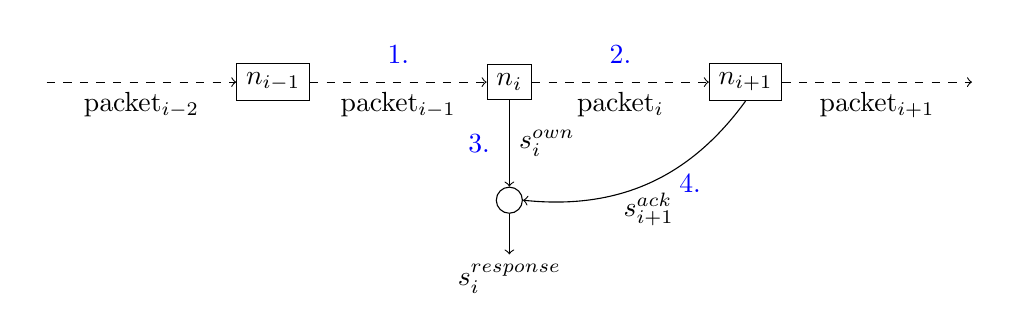
\begin{tikzpicture}[auto]
        \draw (0,0) node (a) {};
        \draw (3.0,0) node (b) [rectangle,draw] {$n_{i-1}$};
        \draw (6,0) node (c) [rectangle,draw] {$n_i$};
        \draw (9.0,0) node (d) [rectangle,draw] {$n_{i+1}$};
        \draw (12.0,0) node (e) {};

        \draw (6.0, -1.5) node [circle,draw] (intermediateResult) {};
        \draw (6.0, -2.5) node (response) {$s_i^{response}$};

        \draw [->,draw,dashed] (a.east) to node [align=center,below] {packet$_{i-2}$} (b.west);
        \draw [->,draw,dashed] (b.east) to node [align=center,below] {packet$_{i-1}$} node [align=center,above,circle] {\color{blue}1.} (c.west);
        \draw [->,draw,dashed] (c.east) to node [align=center,below] {packet$_i$} node [align=center,above,circle] {\color{blue}2.} (d.west);
        \draw [->,draw,dashed] (d.east) to node [align=center,below] {packet$_{i+1}$} (e.west);

        \draw [->,draw] (c.south) to node [right] {$s_i^{own}$} node [align=center,left=1pt,circle] {\color{blue}3.}  (intermediateResult.north);
        \draw [->,draw,bend left] (d.south) to node[below] {$s_{i+1}^{ack}$} node [align=center,right=5pt,circle] {\color{blue}4.} (intermediateResult.east);
        \draw [->,draw] (intermediateResult.south) to (response.north);
    \end{tikzpicture}
    \caption{\color{blue}1. \color{black} Node $n_i$ receives $packet_{i-1}$, validates it, transforms it and \color{blue}2. \color{black} sends it to node $n_{i+1}$. \color{blue}3. \color{black} While processing $packet_i$, node $n_i$ derives $s_i^{own}$ and once node $n_{i+1}$ considered $packet_i$ valid, it \textit{acknowledges} the reception of $packet_i$ and thereby reveals $s_{i+1}^{ack}$ to node $n_i$ which allows node $n_i$ to reconstruct $s_i^{response}$.}
    \label{fig:proofofrelay}
\end{figure}

\paragraph{Challenge-response}

Tickets that that are sent next to a mixnet packet include a challenge $C_i$ which is computed as $$C_i = s_i^{response} \cdot G = (s_i^{own} + s_{i+1}^{ack}) \cdot G$$ where $G$ refers to the base-point and $\cdot$ means scalar multiplication on the curve. Hence, in order to solve the challenge, it is necessary to know $s_i^{own}$ as well as $s_{i+1}^{ack}$.

\paragraph{Challenge and Hint}
\label{sec:proofofrelay:challenge}

Once a node receives a packet, it is able to derive $s_i^{own}$ but it is unable to decide whether $s_{i+i}^{ack}$ will ever lead to $s_i^{response}$ that solves the challenge. Since the underlying field preserves the distributivity, it holds that $$C_i = s_i^{response} \cdot G = (s_i^{own} + s_{i+1}^{ack}) \cdot G = s_i^{own} \cdot G + s_{i+1}^{ack} \cdot G$$

Hence by knowing $hint_i = s_{i+1}^{ack} \cdot G$, the node can verify that $s_i^{own} \cdot G + hint_i = C_i$ and thereby check that the creator of the challenge must have known a value $\tilde{s}_{i+1}^{ack}$ that led to $hint_i$. Due to the infeasibility to invert scalar multiplication on the utilized curve, knwowing $hint_i$ does not reveal $s_{i+1}^{ack}$. Hence, by embedding $hint_i$ into the part of $\beta$ within the SPHINX packet that is readable by node $n_i$, the sender of the makes the validity of the embedded challenge verifiable.

As the next downstream node would not accept a packet without a ticket\footnote{By default, nodes are only forwarding packets that include incentives. Nevertheless, the protocol does not prevent them from processing packets without enforcing an incentive.}, the node $n_i$ does not only need to transform the packet but also issue a ticket to the next downstream node $n_{i+1}$. Therefore, it needs to know \textit{which} challenge $\tilde{C}_{i+1}$ to put into the ticket issued for node $n_{i+1}$. As in the previous section, this is done with the help of the creator of the packet which embeds $C_{i+1}$ into the part of the SPINX packet that is readable by node $n_{i+1}$.

\begin{figure}[H]
    \centering
    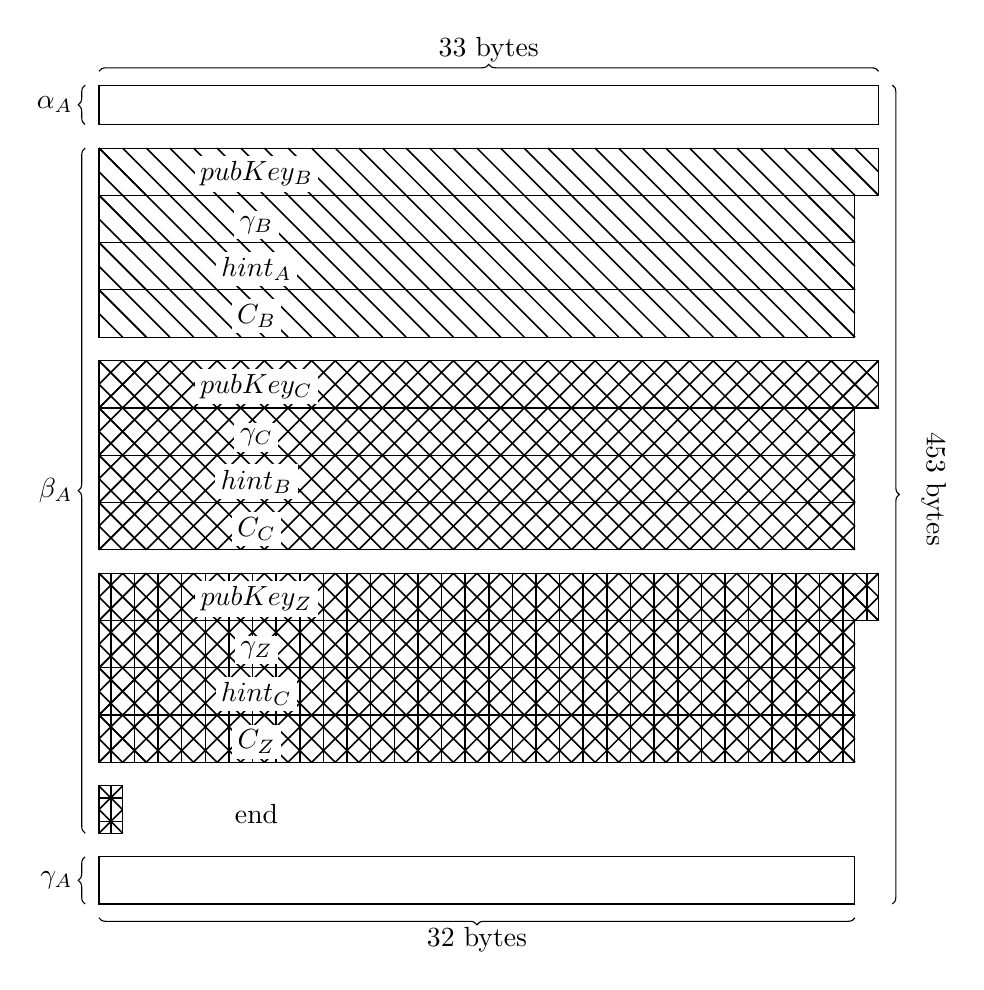
\begin{tikzpicture}
        \def\one{0.3}
        \draw[decoration={brace,raise=5pt},decorate] (0,0.5) -- node[above=5pt] {33 bytes} (33*\one,0.5);
        \draw[decoration={brace,raise=5pt},decorate] (0,0) -- node[left=6pt] {$\alpha_A$} (0,0.5) ;
        \draw[black] (0,0) rectangle (\one*33,0.5);

        \draw[decoration={brace,raise=5pt},decorate] (0,-9.0) -- node[left=6pt] {$\beta_A$} (0,-0.3);

        \foreach \name\length\offset\hatching in{$pubKey_B$/33/-0.9/1,$\gamma_B$/32/-1.5/1,$hint_A$/32/-2.1/1,$C_B$/32/-2.7/1,$pubKey_C$/33/-3.6/2,$\gamma_C$/32/-4.2/2,$hint_B$/32/-4.8/2,$C_C$/32/-5.4/2,$pubKey_Z$/33/-6.3/3,$\gamma_Z$/32/-6.9/3,$hint_C$/32/-7.5/3,$C_Z$/32/-8.1/3}{
                \draw (0,\offset) rectangle (\one*\length,\offset+0.6);
                \begin{scope}[shift={(0,\offset)}]
                    \ifnum\length=33
                        \def\a{9.9}
                        \def\diff{9.4}
                    \else
                        \def\a{9.6}
                        \def\diff{9.1}
                    \fi
                    \def\b{0.6}
                    \def\lw{0.2}

                    \foreach \x [count=\i] in{0,0.3,0.6,...,\b}{
                            \draw [line width=\lw mm](\x,0)--(0,\x) (\a-\b+\x,\b)--(\a,\x);
                        }
                    \foreach \x [count=\i] in{0,0.3,0.6,...,\diff}{
                            \draw [line width=\lw mm](\x+\b,0)--(\x,\b);
                        }

                    \ifnum\hatching>1
                        \foreach \x [count=\i] in{0,0.3,0.6,...,\b}{
                                \draw [line width=\lw mm](0,\x)--(\b-\x,\b) (\a-\b+\x,0)--(\a,\b-\x);
                            }
                        \foreach \x [count=\i] in{0,0.3,0.6,...,\diff}{
                                \draw [line width=\lw mm](\x,0)--(\b+\x,\b);
                            }
                    \fi

                    \ifnum\hatching>2
                        \foreach \x [count=\i] in{0,0.15,0.45,...,\a}{
                                \draw [line width=\lw mm](\x,0)--(\x,\b);
                            }
                    \fi
                \end{scope}

                \draw (2.0,\offset+0.25) node[fill=white,above=-6pt,inner sep=2pt] {\name};

            }

        \draw (0,-8.4) rectangle (\one*1,-9.0);

        \begin{scope}[shift={(0,-9.0)}]
            \def\lw{0.2}

            \draw [line width=\lw mm](0,0)--(0.3,0.3);
            \draw [line width=\lw mm](0,0.3)--(0.3,0.6);

            \draw [line width=\lw mm](0,0.6)--(0.3,0.3);
            \draw [line width=\lw mm](0,0.3)--(0.3,0);

            \draw [line width=\lw mm](0.15,0)--(0.15,0.6);

            \draw [line width=\lw mm](0,0.15)--(0.3,0.15);
            \draw [line width=\lw mm](0,0.45)--(0.3,0.45);

            \draw (2.0,0.25) node[fill=white,above=-7pt] {end};
        \end{scope}

        \draw[decoration={brace,raise=5pt},decorate] (0,-9.9) -- node[left=6pt] {$\gamma_A$} (0,-9.3);

        \draw (0,-9.3) rectangle (\one*32,-9.9);
        \draw[decoration={brace,mirror,raise=5pt},decorate] (0,-9.9) -- node[below=5pt] {32 bytes} (32*\one,-9.9);

        \draw[decoration={brace,raise=5pt},decorate] (33*\one,0.5) -- node[right=12pt,above=2pt,rotate=-90] {453 bytes} (33*\one,-9.9) ;

    \end{tikzpicture}
    \caption{Mixnet packet header with PoR fields that is sent from the sender $O$ through nodes $A, B, C$ to $Z$.}
\end{figure}

By chaining this principle, nodes are forced to \textit{always} issue a ticket to the next downstream node because they are unable to claim their own incentive without the help of the next downstream node.

Since the very last node, namely the final receiver, of the message, does not need to forward the message to anyone else, it has no direct incentive to acknowledge tickets, hence there are no \textit{direct} consequences for \textit{not} acknowledging packet. In its current version, the protocol does not prevent this kind of behavior but it is foreseen to solve this issue by using a reputation system.

\subsection{On-chain Commitment}

HOPR uses a commitment scheme to deposit values on-chain and reveal them once a node redeems an incentive for relaying packets. This comes with the benefit that the redeeming party discloses a secret that is unknown to the issuer of the incentive until it is claimed on-chain. The $opening$ and the $response$ to the PoR challenge are then used by the smart contract to determine whether the ticket has been redeemed or not.

\begin{defnsub}
    % Currently leaving out further details such as unconditionally/computationally binding / hiding
    A commitment scheme $Cm = (\mathsf{Commit}, \mathsf{Open})$ is a protocol between two parties, $A$ and $B$, that gives $A$ the opportunity to store a value $comm = \mathsf{Commit}(x)$ at $B$. The value $x$ stays unknown to $B$ until $A$ decides to reveal it to $B$.

    \noindent\textbf{Hiding:} A commitment scheme is called \textbf{hiding} if it is infeasible for an adversary $\mathsf{Adv}$ to recover $x$ from $comm$.

    \noindent\textbf{Binding:} A commitment scheme is called \textbf{binding} if it is infeasible for an adversary $\mathsf{Adv}$ to find a value $x'$ with $x \neq x'$ such that $\mathsf{Open}(cm, x') \neq \bot$.
\end{defnsub}

\subsubsection{Setup phase}

Once a node engages with another node in a payment channel and lock funds within that channel, it derives a master key $comm_0$ from its private key and uses it to create an iterated commitment $comm_i$ such that for every $i \in \mathbb{N}_0$ and $i > 0$ it holds that $$ \mathsf{Open}(comm_{i}, comm_{i-1}) = \top $$
The iterated commitment is computed as $$comm_n = hash^n(comm_0)$$ where $\mathsf{hash}$ is a preimage-resistant hash function and $comm_0$ is derived as 
$$ comm_0 = \mathsf{hash}(privKey, chainId, contractAddr, channelId, channelEpoch)$$
The master key is supposed to be pseudo-random such that all intermediate commitments $comm_{i}$ for $i \in \mathbb{N}_0$ and $0 < i \le n$ are indistinguishable for the ticket issuer from random numbers of the same length. This is necessary in order to ensure that the ticket issuer is unable to determine whether a ticket is a win or not when issuing the ticket. This makes it infeasible for the ticket issuer to tweak the challenge to such that it cannot be a win.
\\~\\When dispatching a transaction that opens the payment channel, the commitment $comm_n$ is stored in the channel structure in the smart contract and the smart contract will force the ticket recipient to reveal $comm_{n-1}$ when redeeming a ticket issued in this channel.
The number of iterations $n$ can be chosen as a constant and should reflect the number of tickets a node intends to redeem within a channel.

\subsubsection{Opening phase}

In order to redeem a ticket, a node has to reveal the opening to the current commitment $comm_i$ that is stored in the smart contract for the channel. Since the opening $comm_{i-1}$ allows the ticket issuer to determine whether a ticket is going to be a win, the ticket recipient should keep $comm_{i-1}$ until it is used to redeem a ticket.
Tickets lead to a win if $\mathsf{hash}( t_h, r, comm_{i-1} ) < P_w$ where $t_h=\mathsf{hash}(t)$ and $\mathsf{Open}(comm_i, comm_{i-1}) = \top$. Since $comm_{0}$ is known to the ticket recipient, the ticket recipient can compute the opening as $comm_{n-1} = \mathsf{hash}^{n-1}(comm_0)$.
Once redeeming a ticket, the smart contract verifies that $$\mathsf{Open}(comm_i, comm_{i-1}) = \top$$ and sets $channel.comm[redeemer] \leftarrow comm_{i-1}$. Hence next time, the node redeems a ticket, it has to reveal $comm_{i-2}$.
In addition, each node is granted the right to reset the commitment to a new value which is necessary especially once a node reveals $comm_0$ and therefore is with high probability unable to compute a value $r$ such that $$\mathsf{Open}(comm_0,r) \neq \bot$$
Since this mechanism can be abused by the ticket recipient to tweak the entropy that is used to determine whether a ticket is a win or not, the smart contract keeps track on resets of the on-chain commitment and sets $$channel.ticketEpoc[redeemer] \leftarrow channel.ticketEpoc[redeemer] + 1$$ and thereby invalidates all previously unredeemed tickets.




\subsection{Probabilistic Payment Channels}
\label{sec:incentives:probabilistic}

Payment channels give two nodes, $A$ and $B$, the opportunity to lock funds on-chain and later on handle who of them possesses which fraction. At each moment, it holds that

$$ balance(A) + balance(B) = const. $$

The state becomes final once one of the nodes submits the most recent state to the smart contract. Therefore it requires a proof by the counterparty that the proclaimed state is in their interest, which is given by a digital signature and named \textit{update transaction}. Hence an update transaction that transfers $x > 0$ digital assets from $A$ to $B$ is approved by,

$$ update_i = Sig_A (balance(A) - x \ || \ balance(B) + x) $$

By doing so, payments can only in one direction, turning the payment channel into a unidirectional payment channel. This is possible because digital assets will only be transferred from $A$ to $B$ and thus $B$ will always pick in its own the interest the most recent update transaction since $balance(B)$ is strictly increasing.

If the channel allowed asset transfers in the opposite direction, namely from $B$ to $A$ the update transactions need to include a versioning element that prevents any of the parties from rollback to the most beneficial state since the smart contract is unable to determine the most recent transaction otherwise. Hence,

$$ update_i = Sig_A (i \ || \ balance(A) - x \ || \ balance(B) + x) $$

In addition, this requires certain timeframes in which the counterparty is given the opportunity to present their most recent update update transaction. This is necessary because none of the nodes can prove that there does \textit{not} exist a more recent update transaction. Once the timeout ends, and none of the parties have submitted any more recent update transaction, the last submitted state becomes final.

\begin{figure}[H]
    \centering
    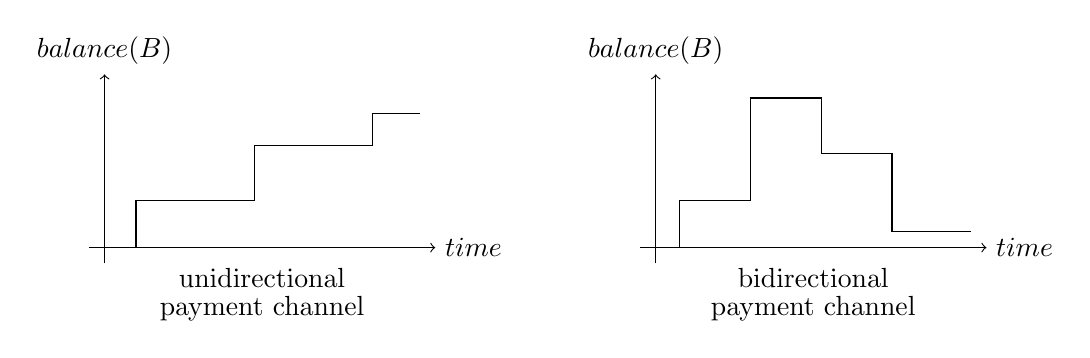
\begin{tikzpicture}[domain=0:2]
        \def\padding{0.1}
        \def\plotHeight{2}
        \def\plotWidth{4}
        \def\plotOffset{7}
        \def\textOffset{0.6}
        \foreach \i in {0,1} {
                \begin{scope}[shift={(\i*\plotOffset,0)}]
                    \draw[->] (-2*\padding,0) -- (\plotWidth+2*\padding,0) node[right] {$time$};
                    \draw[->] (0,-2*\padding) -- (0,\plotHeight+2*\padding) node[above] {$balance(B)$};

                    \ifnum\i=0
                        \path (0,-\textOffset) -- (\plotWidth,-\textOffset) node[midway] {\shortstack{unidirectional\\payment channel}};
                        \draw (0.4,0) -- (0.4,0.6) -- (1.4,0.6) -- (1.9,0.6) -- (1.9,1.3) -- (2.6,1.3) -- (3.4,1.3) -- (3.4,1.7) -- (4.0,1.7);
                    \else
                        \path (0,-\textOffset) -- (\plotWidth,-\textOffset) node[midway] {\shortstack{bidirectional\\payment channel}};

                        \draw (0.3,0) -- (0.3,0.6) -- (1.2,0.6) -- (1.2,1.9) -- (2.1,1.9) -- (2.1,1.2) -- (3.0,1.2) -- (3.0,0.2) -- (4.0,0.2);
                    \fi
                \end{scope}
            }
    \end{tikzpicture}
    \label{fig:channels}
    \caption{Node $A$ and $B$ have a payment channel. Whilst in case of unidirectional payment channels, $balance(B)$ is strictly increasing, the derivative of $balance(B)$ \textit{can} change sign if the channel is bidirectional.}
\end{figure}

Within the HOPR protocol, payment channels are implemented as unidirectional channels, hence there \textit{can} be one from $A \rightarrow B$ and another one from $B \rightarrow A$. Whenever, an update transaction is submitted to the blockchain, the assets get transferred to the channel in the opposite direction, or directly to the counterparty if there is no such channel. This obviously controverses the original purpose of payment channels, which is \textit{aggregation} of asset transfers.

When talking about unidirectional payment channels, aggregation means that $value(update_i) = value(update_{i-1}) + \Delta x$, hence $update_i$ makes $update_{i-1}$ obsolete as it already includes the additional assets $\Delta x$. So, if a node manages to receive $update_i$ before $update_{i-1}$, there is no need to provide the services the which were supposed to be compensated by $update_{i-1}$.

This is problematic for HOPR because it uses \nameref{sec:incentives:proofofrelay} to unlock payment made from one node to the other and the state of a payment channel between nodes $n_{i-1}$ and $n_i$ therefore relies on third-party actions, namely by $n_{i+1}$ and $n_{i+1}'$. Both of them acknowledge the reception of the packet and the correct transformation done by node $n_i$. Using update transactions arises the question which update transaction node $n_{i+1}$ and node $n_{i+1}'$ should sign because they cannot know which acknowledgement reaches $n_i$ first. Hence, the incentives for packet need to be done independently and thus should not rely on update transactions.

\begin{figure}[H]
    \centering
    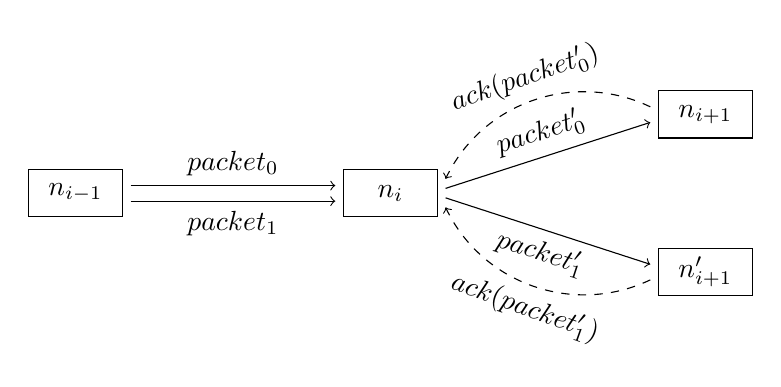
\begin{tikzpicture}
        \def\nodeOffset{4}
        \def\nodeYOffset{1}
        \def\nodeWidth{1.2}
        \def\nodeHeight{0.6}
        \def\padding{0.1}

        \foreach \xOffset\yOffset\name in{-\nodeOffset/0/$n_{i-1}$,0/0/$n_i$,\nodeOffset/\nodeYOffset/$n_{i+1}$,\nodeOffset/-\nodeYOffset/$n_{i+1}'$} {
                \draw[shift={(\xOffset,\yOffset)}] (0,0) rectangle (\nodeWidth,\nodeHeight) node[midway] {\name};
            }

        % Packets
        \draw[->,shift={(0,0.66*\nodeHeight)}] (-\nodeOffset+\nodeWidth+\padding,0) -- (-\padding,0) node[midway,above] {$packet_0$};
        \draw[->,shift={(0,0.33*\nodeHeight)}] (-\nodeOffset+\nodeWidth+\padding,0) -- (-\padding,0) node[midway,below] {$packet_1$};

        % Forwarded packets
        \draw[->] (\nodeWidth+\padding,0.6*\nodeHeight) -- (\nodeOffset-\padding,\nodeYOffset+0.33*\nodeHeight) node[midway,sloped,above] {$packet_0'$};
        \draw[->] (\nodeWidth+\padding,0.4*\nodeHeight) -- (\nodeOffset-\padding,-\nodeYOffset+0.66*\nodeHeight) node[midway,sloped,below] {$packet_1'$};

        % Acknowledgements
        \draw[->,dashed] (\nodeOffset-\padding,\nodeYOffset+0.66*\nodeHeight) to [bend right=45] node[above,sloped] {$ack(packet_0')$} (\nodeWidth+\padding,0.8*\nodeHeight);
        \draw[->,dashed] (\nodeOffset-\padding,-\nodeYOffset+0.33*\nodeHeight) to [bend left=45] node[below,sloped] {$ack(packet_1')$} (\nodeWidth+\padding,0.2*\nodeHeight);
    \end{tikzpicture}
    \caption{Node $n_{i-1}$ send packet $packet_0$, $packet_1$ to node $n_i$ which forwards them to node $n_{i+1}$ and node $n_{i+1}'$. Both nodes acknowledge the validity of $packet_0'$ and $packet_1'$ to node $n_i$.}
    \label{fig:sharedpaymentchannel}
\end{figure}

\paragraph{Probabilistic payments}
\label{sec:incentives:probabilistic:probabilistic}

Incentives relate to packets which are assumed to be sent very often in the HOPR network. Nodes can therefore expect that they will shortly receive another micropayment from the same node. It is thus not necessary to claim the incentive for each packet individually. This is why nodes issue each other probabilistic \lcnameref{sec:tickets} that have the same asymptotic payout but do neither require in-order processing nor require an on-chain operation for every incentive. Hence when picking the same relay fee, it holds that

$$ \forall i \ \forall j \ : \ value(ticket_i) = value(ticket_j) $$

Moreover, the nodes estimate the usage of the link to the nodes with whom they have engaged in a payment channel and pick a ticket winning probability that leads to a continous payout. Connections with higher througput can use lower probabilities whilst those with fewer traffic are supposed to use winning probabilities closer to 1.

Probabilistic payments rely on the necessity for the ticket issuer to not know whether a ticket that is issued will turn into an asset transfer or not. Hence, the ticket redemption must rely on some entropy provided by the ticket redeemer and need to be kept secret until the ticket is redeemed. This is necessary, because by knowing which ticket is going to become a winner, the ticket issuer would solely issue losing tickets and thereby withhold the incentives for the next downstream node.

Analogously, the ticket receiver should not know whether a ticket will be a win before being able to reconstruct the response to the challenge stated in the ticket. If not, the ticket receiver would just process those packet that come with a winning ticket and drop all other packets.

A ticket is a winner if

$$ keccak256 ( ticketHash \ || \ porSecret \ || \ opening) < ticket.invWinProb $$

where $ticketHash$ is the hash of the received ticket, see section \ref{sec:tickets:redemption}, and thus known by both ticket issuer and recipient whereas $porSecret$ is known by the ticket issuer and can be reconstructed as part of the $\nameref{sec:incentives:proofofrelay}$ scheme by the ticket recipient once it receives the acknowledgement for the forwarded ticket. On the other hand, $opening$ refers to the value that opens the most recent commitment that is stored on-chain, see section \ref{sec:incentives:commitment}. The on-chain commitment is chosen by the ticket recipient and due to the hiding property of the utilized commitment scheme, the opening values are solely known by the ticket recipient.
